\scanpage{22}
On est ramené au cas $U=X$, soit $A$ qui est loc. une réunion de feuilles, l'est-il globalement? Il suffit de prouver que pour tte feuille $X_i$, telle que $X_i\cap A\ne\varnothing$, on a $X_i\subset A$, ou encore que $X_i\cap A$ est une partie à la fois ouverte et fermée de $A$. C'est une condition locale sur $X$, or loc. sur $X$ $A$ est \unsure{comme|connue} une réunion de feuilles, OK!

Cet argument montre plus gén. que pour \uline{tout} ouvert $U\subset X$, si $A\in\overline F_U$, alors les $A\unsure{\cap|\equiv} X_i$ sont à la fois ouverts et fermés dans $X_i\cap U$, donc des réunions des comp. connexes de $X_i\cap U$. \inserted{Donc $A$ est réunion de comp. connexes d'ens. \deleted{\unsure{ouverts}} de la forme $X_i\cap U$.} Inversement, supposons que $A$ soit une telle réunion, cela implique-t-il que $A\in\overline F_U$? \deleted{Evidemment, \unsure{les composantes}}\inserted{En particulier, une comp.} connexe d'un $X_i\cap U$ est-il $\in\overline F_U$?

\uuline{Non}, exemple:
\[
\begin{aligned}
&X=U=\text{droite numérique }\mathbb R\\
&\deleted{\unsure{F}=\{\varnothing,\mathbb R,\{0\},\mathbb R^*\}}\\
&X_0=\{0\},\quad X_1=\mathbb R^*=\mathbb R-\{0\}
\end{aligned}
\]
\figure{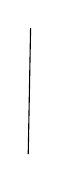
\begin{tikzpicture}[x=1cm,y=1cm]\draw (0,0)--(0.03,1.6);\end{tikzpicture}}
$\mathbb R^+$ n'est pas $\in\overline F=F_X$.

\figure{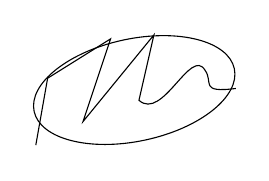
\begin{tikzpicture}[x=1cm,y=1cm]\draw[rotate=12] (0,0) ellipse (1.3 and .65);\draw (-1.25,-.7)--(-1.1,.15)--(-.3,.65)--(-.65,-.4)--(.25,.7)--(.06,-.13) .. controls (.36,-.4) and (.72,.56) .. (.9,.25) .. controls (1.01,.1) and (.82,-.04) .. (1.29,.02);\end{tikzpicture}}

Si on veut un exemple avec des $X_i$ connexes, $U\ne X$, on prend $X=\widehat{\mathbb R}=\unsure{\mathbb P^1_{\mathbb R}|\mathbb S^1}$; \deleted{$\unsure{U\in F}$} $X_0=\{0\}$, $X_1=X-\{0\}$, $U=\mathbb R$ ---
\mspage{23}
